\documentclass{standalone}

\usepackage{pgfplots,tikz,amsmath}
\begin{document}
    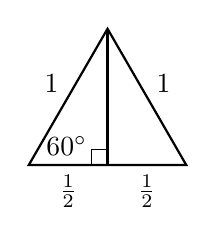
\begin{tikzpicture}
        \draw[black, thick] (0,0) -- (2,0) -- (1,1.73) -- cycle;
        \draw[black, thick] (1,0) -- (1,1.73);
        \draw[black] (0.8,0) -- (0.8,0.2) -- (1,0.2);
        \draw (0.5,0) node[anchor=north]{$\frac{1}{2}$};
        \draw (1.5,0) node[anchor=north]{$\frac{1}{2}$};
        \draw (0.5,0.8) node[anchor=south east]{$1$};
        \draw (1.5,0.8) node[anchor=south west]{$1$};
        \draw (0.1,0) node[anchor=south west]{$60^\circ$};
    \end{tikzpicture}
    \hspace{1in}
    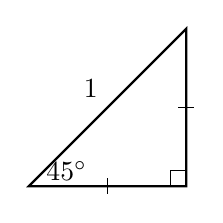
\begin{tikzpicture}
        \draw[black, thick] (0,0) -- (2,0) -- (2,2) -- cycle;
        \draw[black] (1.8,0) -- (1.8,0.2) -- (2,0.2);
        \draw[black] (1,0.1) -- (1,-0.1);
        \draw[black] (1.9,1) -- (2.1,1);
        \draw (1,1) node[anchor=south east]{$1$};
        \draw (0.1,-0.05) node[anchor=south west]{$45^\circ$};
    \end{tikzpicture}
\end{document}
